\documentclass{article}

% For adjusting images
\usepackage{adjustbox}
% For functions like \binom
\usepackage{amsmath}
% For functions like \wedge \subseteq \mathbb
\usepackage{amssymb}
% 312 Font
\usepackage{charter}
% Circuit diagrams
\usepackage{circuitikz}
% Custom lists
\usepackage{enumitem}
% Page margins & pagestyles
\usepackage{fullpage}
% Font encoding
\usepackage[T1]{fontenc}
% Used in 7-segment display
\usepackage{ifthen}
% Colored boxes around the 'solution' environment
\usepackage{mdframed}
% Used for making 7-segment displays
\usepackage{tikz}
\usetikzlibrary{calc}
% For color
\usepackage[dvipsnames]{xcolor}

% Defines a solution environment that creates a green box around text inside.
\mdfdefinestyle{SolutionFrame}{linecolor=green!60!black,linewidth=1pt}
\newenvironment{solution}{\begin{mdframed}[style=SolutionFrame]}{\end{mdframed}}

% Enumerate with (a),(b),(c),...
\newenvironment{enum}{\begin{enumerate}[label={(\alph*)}]}{\end{enumerate}}

% Put a dot after section titles
\renewcommand\thesection{\arabic{section}.}
\renewcommand\thesubsection{\arabic{section}.\arabic{subsection}}

% Hide the Date
\date{}
% Hide page numbers
\pagenumbering{gobble}

\begin{document}
    % Used for making 7-Segment Displays
    % \documentclass[preview,varwidth]{standalone}

% \usepackage{mdframed}
% \usepackage{ifthen}
% \usepackage{tikz}
% \usetikzlibrary{calc}

\pgfkeys{
    /sevenseg/.is family, /sevenseg,
    slant/.estore in      = \sevensegSlant,     % vertical slant in degrees
    size/.estore in       = \sevensegSize,      % length of a segment
    shrink/.estore in     = \sevensegShrink,    % avoids overlapping of segments
    line width/.estore in = \sevensegLinewidth, % thickness of the segments
    line cap/.estore in   = \sevensegLinecap,   % end cap style rect, round, butt
    oncolor/.estore in    = \sevensegOncolor,   % color of an ON segment
    offcolor/.estore in   = \sevensegOffcolor,  % color of an OFF segment
}

\pgfkeys{
    /sevenseg,
    default/.style = {
        slant = 0,
        size = 4em,
        shrink = 0.1, 
        line width = .75em,
        line cap = butt, 
        oncolor = red,
        offcolor = black!75
    }
}

%                     a b c d e f g - segment values
% \sevenseg[options]{{1,1,1,1,1,1,0,}}
\newcommand{\sevenseg}[2][] {
    \pgfkeys{/sevenseg, default, #1}
    \def\sevensegarray{#2}
    \begin{tikzpicture}
        % first define the position of the 6 corner points
        \path (0,0) ++(0,0)                             coordinate (P1);
        \path (0,0) ++(\sevensegSize,0)                 coordinate (P2);
        \path (0,0) ++(90-\sevensegSlant:\sevensegSize) coordinate (P3);
        \path (P2)  ++(90-\sevensegSlant:\sevensegSize) coordinate (P4);
        \path (P3)  ++(90-\sevensegSlant:\sevensegSize) coordinate (P5);
        \path (P4)  ++(90-\sevensegSlant:\sevensegSize) coordinate (P6);
        
        % then step through the 1/0 values in the segment array
        \foreach \i in {0,...,6} {
            \pgfmathparse{\sevensegarray[\i]}
            \ifthenelse{\equal{\pgfmathresult}{1}}
                {\let\mycolor=\sevensegOncolor}     % segment is on
                {\let\mycolor=\sevensegOffcolor}    % segment is off
            \tikzstyle{segstyle} = [draw=\mycolor, line width = \sevensegLinewidth,
                                  line cap = \sevensegLinecap]

            \ifthenelse{\equal{\i}{0}}{\path[segstyle] 
                (${1-\sevensegShrink}*(P5)+\sevensegShrink*(P6)$) 
                -- ($\sevensegShrink*(P5)+{1-\sevensegShrink}*(P6)$);}{} % a
            \ifthenelse{\equal{\i}{1}}{\path[segstyle] 
                (${1-\sevensegShrink}*(P6)+\sevensegShrink*(P4)$) 
                -- ($\sevensegShrink*(P6)+{1-\sevensegShrink}*(P4)$);}{} % b
            \ifthenelse{\equal{\i}{2}}{\path[segstyle] 
                (${1-\sevensegShrink}*(P4)+\sevensegShrink*(P2)$) 
                -- ($\sevensegShrink*(P4)+{1-\sevensegShrink}*(P2)$);}{} % c
            \ifthenelse{\equal{\i}{3}}{\path[segstyle] 
                (${1-\sevensegShrink}*(P1)+\sevensegShrink*(P2)$) 
                -- ($\sevensegShrink*(P1)+{1-\sevensegShrink}*(P2)$);}{} % d
            \ifthenelse{\equal{\i}{4}}{\path[segstyle] 
                (${1-\sevensegShrink}*(P1)+\sevensegShrink*(P3)$) 
                -- ($\sevensegShrink*(P1)+{1-\sevensegShrink}*(P3)$);}{} % e
            \ifthenelse{\equal{\i}{5}}{\path[segstyle] 
                (${1-\sevensegShrink}*(P3)+\sevensegShrink*(P5)$) 
                -- ($\sevensegShrink*(P3)+{1-\sevensegShrink}*(P5)$);}{} % f
            \ifthenelse{\equal{\i}{6}}{\path[segstyle] 
                (${1-\sevensegShrink}*(P3)+\sevensegShrink*(P4)$) 
                -- ($\sevensegShrink*(P3)+{1-\sevensegShrink}*(P4)$);}{} % g
        }
  \end{tikzpicture}
}

% Examples (Uncomment document type & packages at the top of the file too)
% \begin{document}
%     \begin{mdframed}[backgroundcolor=black]
%         \begin{center}
%             \sevenseg{{1,0,0,0,0,0,0}} \quad
%             \sevenseg{{0,1,0,0,0,0,0}} \quad
%             \sevenseg{{0,0,1,0,0,0,0}} \quad
%             \sevenseg{{0,0,0,1,0,0,0}} \quad
%             \sevenseg{{0,0,0,0,1,0,0}} \quad
%             \sevenseg{{0,0,0,0,0,1,0}} \quad
%             \sevenseg{{0,0,0,0,0,0,1}}
%         \end{center}
%     \end{mdframed}
%     \vspace{10pt}
%     \begin{mdframed}[backgroundcolor=black]
%         \begin{center}
%             \sevenseg{{1,1,1,1,1,1,0}} \quad
%             \sevenseg{{0,1,1,0,0,0,0}} \quad
%             \sevenseg{{1,1,0,1,1,0,1}} \quad
%             \sevenseg{{1,1,1,1,0,0,1}} \vspace{10pt} \\
%             \sevenseg{{0,1,1,0,0,1,1}} \quad
%             \sevenseg{{1,0,1,1,0,1,1}} \quad
%             \sevenseg{{1,0,1,1,1,1,1}} \quad
%             \sevenseg{{1,1,1,0,0,0,0}} \vspace{10pt} \\
%             \sevenseg{{1,1,1,1,1,1,1}} \quad
%             \sevenseg{{1,1,1,1,0,1,1}}
%         \end{center}
%     \end{mdframed}
% \end{document}
    
    \begin{titlepage}
        \centering
        \null
        \vspace{5cm}
        {\Huge CSE 369 Lab 4\par}
        \vspace{0.5cm}
        {\Large High-Level Verilog \par}
        \vfill
        {\hfill \Large Isaac Wu \par}
        {\hfill \large 2360957 \par}
        {\hfill \large \today \par}
    \end{titlepage}

\section{Item Table}
    \begin{solution}
        \begin{center}
        \Large\begin{tabular}{c|c|c|c}
            Item Name & UPC & Discounted? & Expensive? \\ \hline
            Banana & 0 0 0 & No & Yes \\ \hline
            Bottle & 0 0 1 & No & No \\ \hline
            Needle & 0 1 1 & Yes & No \\ \hline
            Pencil & 1 0 0 & No & Yes \\ \hline
            Spring & 1 0 1 & Yes & Yes \\ \hline
            Sponge & 1 1 0 & Yes & No \\ \hline
        \end{tabular}
        \end{center}
    \end{solution}

\section{ModelSim Simulations}
    \begin{enum}
        \item Double 7-Segment Display
            \begin{solution}
                Here is the code for my double 7-segment display. I defined logic variables for the output of the seg7 module calls to explicitly invert them. The HEX outputs on our DE1s are active low, necessitating the inversion here. I called seg7 twice, once for each digit we want to output with their defined range of switches (3-0 for the first, 7-4 for the second). I then assigned the inverses of the outputs to their corresponding HEX displays on the DE1 board. \\
                \begin{minipage}[t]{0.9\linewidth}
                    \begin{center}
                        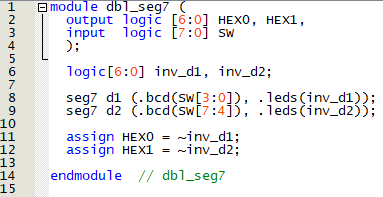
\includegraphics[width=0.9\linewidth]{Lab4/dbl_seg7.png}
                    \end{center}
                \end{minipage}
                
                \newpage
                This is the code for the double 7-segment display test benchmark used to ensure correct functionality from my code. This benchmark will run my dbl\_seg7 module with all 256 combinations of switch inputs. \\
                \begin{minipage}[t]{0.9\linewidth}
                    \begin{center}
                        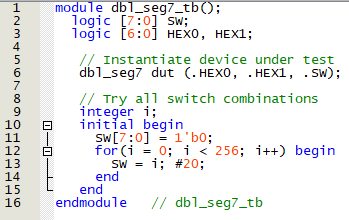
\includegraphics[width=0.9\linewidth]{Lab4/dbl_seg7_tb.png}
                    \end{center}
                \end{minipage}
                
                \clearpage
                This is what my wave diagram looks like. The top 8 waves show the 8 switches alternating to test all 256 combinations. The bottom two waves are the HEX outputs, with HEX0 corresponding to switches 3-0 and HEX1 corresponding to switches 7-4. The binary sequences shown on the wave diagram correspond to the pre-defined display of the switch combination number. Because we are only displaying numbers 0-9, we have some switch combinations we don't care about, which are the red lines shown in the HEX outputs. \\
                \begin{minipage}[t]{0.9\linewidth}
                    \begin{center}
                        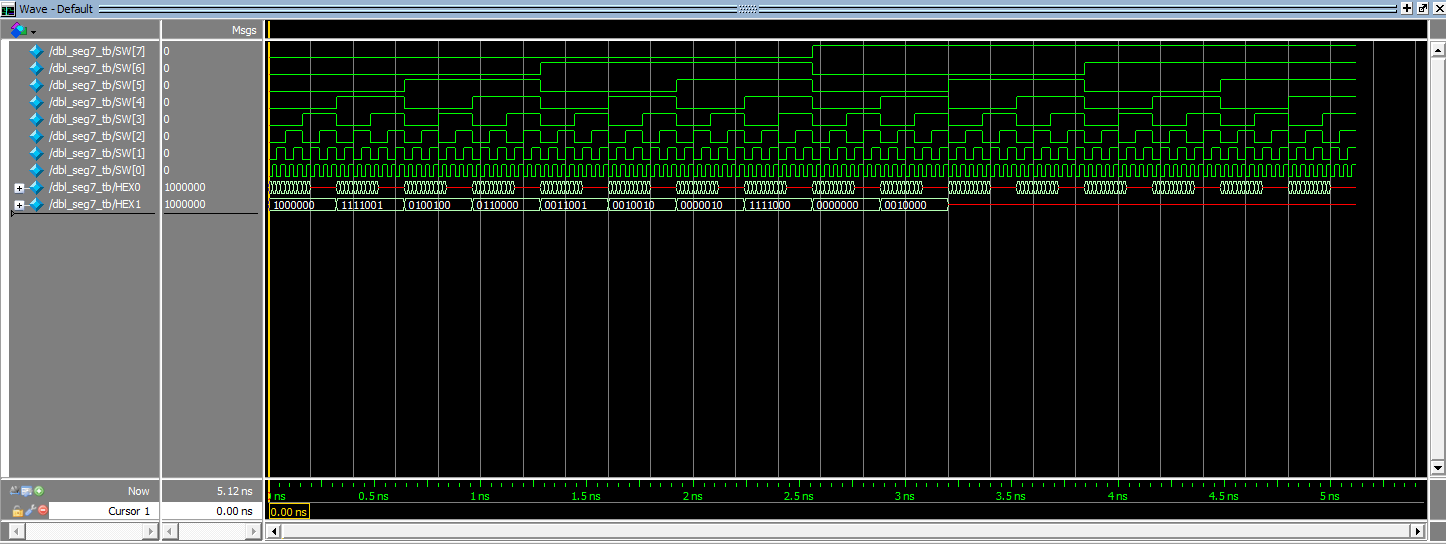
\includegraphics[width=1.1\linewidth]{Lab4/dbl_seg7_waves.png}
                    \end{center}
                \end{minipage}
            \end{solution}

        \newpage
        \item Fred's Pawn Shop
            \begin{solution}
                Here is the code for Lab 4, or Fred's Pawn Shop. I call lab3 to calculate if the item was on sale or stolen using the input switches and outputs to two LEDs. I then call my module display to display the name of the item on the HEX display. I only need the switches corresponding to the UPC number for the display, so I slice the switches array for this input. \\
                \begin{minipage}[t]{0.9\linewidth}
                    \begin{center}
                        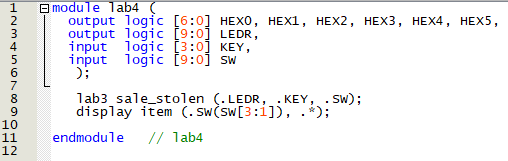
\includegraphics[width=1.0\linewidth]{Lab4/lab4.png}
                    \end{center}
                \end{minipage}

                Here is a revised version of my code from Lab 3, which calculates whether an item was on sale or stolen using the item's UPC code and a Mark input from switches and outputs to two LEDs. I removed the code that would set the HEX displays to their default value (off) since I would be using them to display the item name and the assignment would conflict. I also swapped the LED outputs of Discounted and Stolen to better match the situation. \\
                \begin{minipage}[t]{0.9\linewidth}
                    \begin{center}
                        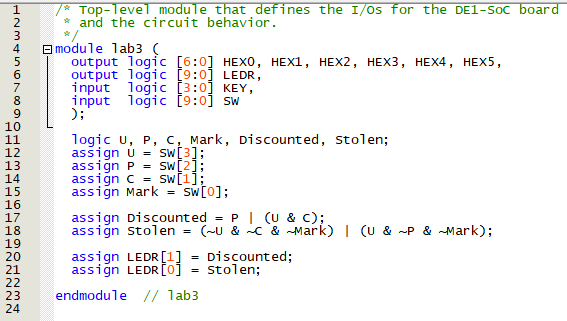
\includegraphics[width=1.0\linewidth]{Lab4/lab3.png}
                    \end{center}
                \end{minipage}

                Here is my display code. This simple module takes in the UPC code of the item and uses a switch-case statement to then assign predetermined values to the HEX displays to display the name of the item. With 8 UPC codes and 6 items, there are two codes that we don't care about, and those are handled in the default case. \\
                \begin{minipage}[t]{0.9\linewidth}
                    \begin{center}
                        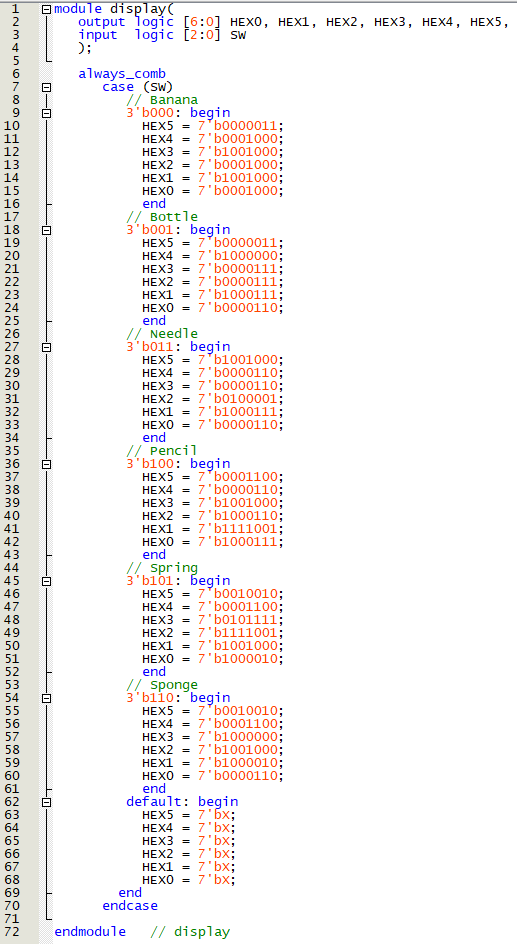
\includegraphics[width=1.0\linewidth]{Lab4/display.png}
                    \end{center}
                \end{minipage}

                This is the code for the test benchmark used to ensure correct functionality from Fred's Pawn Shop. This benchmark will run my lab4 module with all 16 combinations of switch inputs, representing all 8 UPC codes and the Mark input. \\
                \begin{minipage}[t]{0.9\linewidth}
                    \begin{center}
                        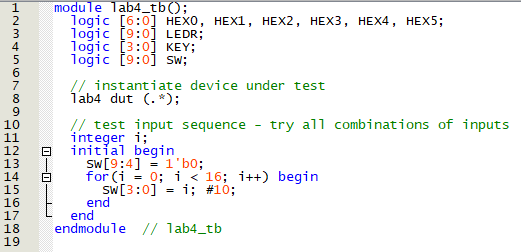
\includegraphics[width=1.0\linewidth]{Lab4/lab4_tb.png}
                    \end{center}
                \end{minipage}

                \clearpage
                This is what the resulting wave diagram looks like. The top 4 waves show the 4 switches alternating to test all 16 combinations. The middle two waves are the LED output, with LEDR[0] corresponding to if a product is Discounted, and LEDR[1] if a product was stolen. The bottom 6 waves are the HEX displays, that show, in order, the pre-programmed letters codes for the 7-segment displays encoded in binary that correspond to the UPC code. \\
                \begin{minipage}[t]{0.9\linewidth}
                    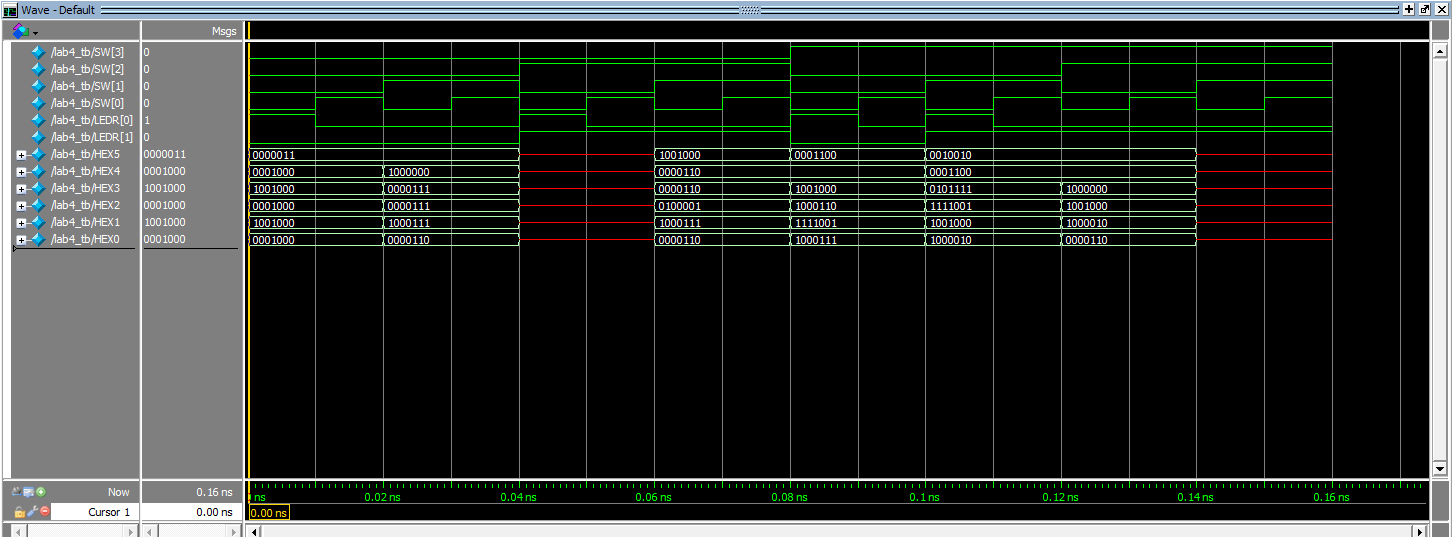
\includegraphics[width=1.1\linewidth]{Lab4/item_waves.png}
                \end{minipage}
            \end{solution}
    \end{enum}

\newpage
\section{Unused UPC 7-Segment Display Outputs}
    \begin{enum}
        \item UPC = 010
            \begin{mdframed}[style=SolutionFrame, backgroundcolor=black]
                \begin{center}
                    \sevenseg{{1,1,1,1,1,1,0}} \quad
                    \sevenseg{{1,1,0,1,1,1,1}} \quad
                    \sevenseg{{1,1,1,1,1,1,0}} \quad
                    \sevenseg{{1,1,1,1,1,1,1}} \quad
                    \sevenseg{{1,0,1,1,1,1,0}} \quad
                    \sevenseg{{1,1,1,0,1,1,1}}
                \end{center}
            \end{mdframed}
        \item UPC = 111
            \begin{mdframed}[style=SolutionFrame, backgroundcolor=black]
                \begin{center}
                    \sevenseg{{1,1,1,1,1,1,1}} \quad
                    \sevenseg{{1,1,0,1,1,1,1}} \quad
                    \sevenseg{{1,0,0,1,1,0,1}} \quad
                    \sevenseg{{0,1,1,1,0,1,0}} \quad
                    \sevenseg{{1,0,1,1,1,1,0}} \quad
                    \sevenseg{{1,0,1,1,1,1,1}}
                \end{center}
            \end{mdframed}
    \end{enum}

\section{Misc.}
    How many hours (estimated) it took to complete this lab in total, including reading, planning, designing, coding, debugging, and testing.
    \begin{solution}
        It took around 5 hours to complete this lab.
    \end{solution}

\end{document}